\chapter{Connecting Database}
For real time database I used firabase real time database system.Because Firebase offers easy integration with various platforms and frameworks and Firebase allows us to extend application's functionality with serverless Cloud Functions.

\section{Steps for creating real time database in Firebase}
Navigate to the Realtime Database section of the Firebase console.And select create new database.Then I needed to install raspbbery some libraries for communicating with database

\subsection{Install to raspberry}
Firstly install pyrabase with this command pip install pyrebase. Then get required informations and fill this parts config\\
    "apiKey"\\
    "authDomain"\\
    "databaseURL"\\
    "storageBucket"\\

With this informations raspi easily interact with firebase. For getting key we need to create add an user to authentication then we get api key and connect easily.

\subsection{Usage}
With adding required codes to main program, we add customers and products to our database.And send count of products to database. If count of product in minibar is reduced in a time(user take a product from minibar), raspberry detects that and decrease count of product and updates customers bill.
\begin{figure}[!htbp]
    \centering
    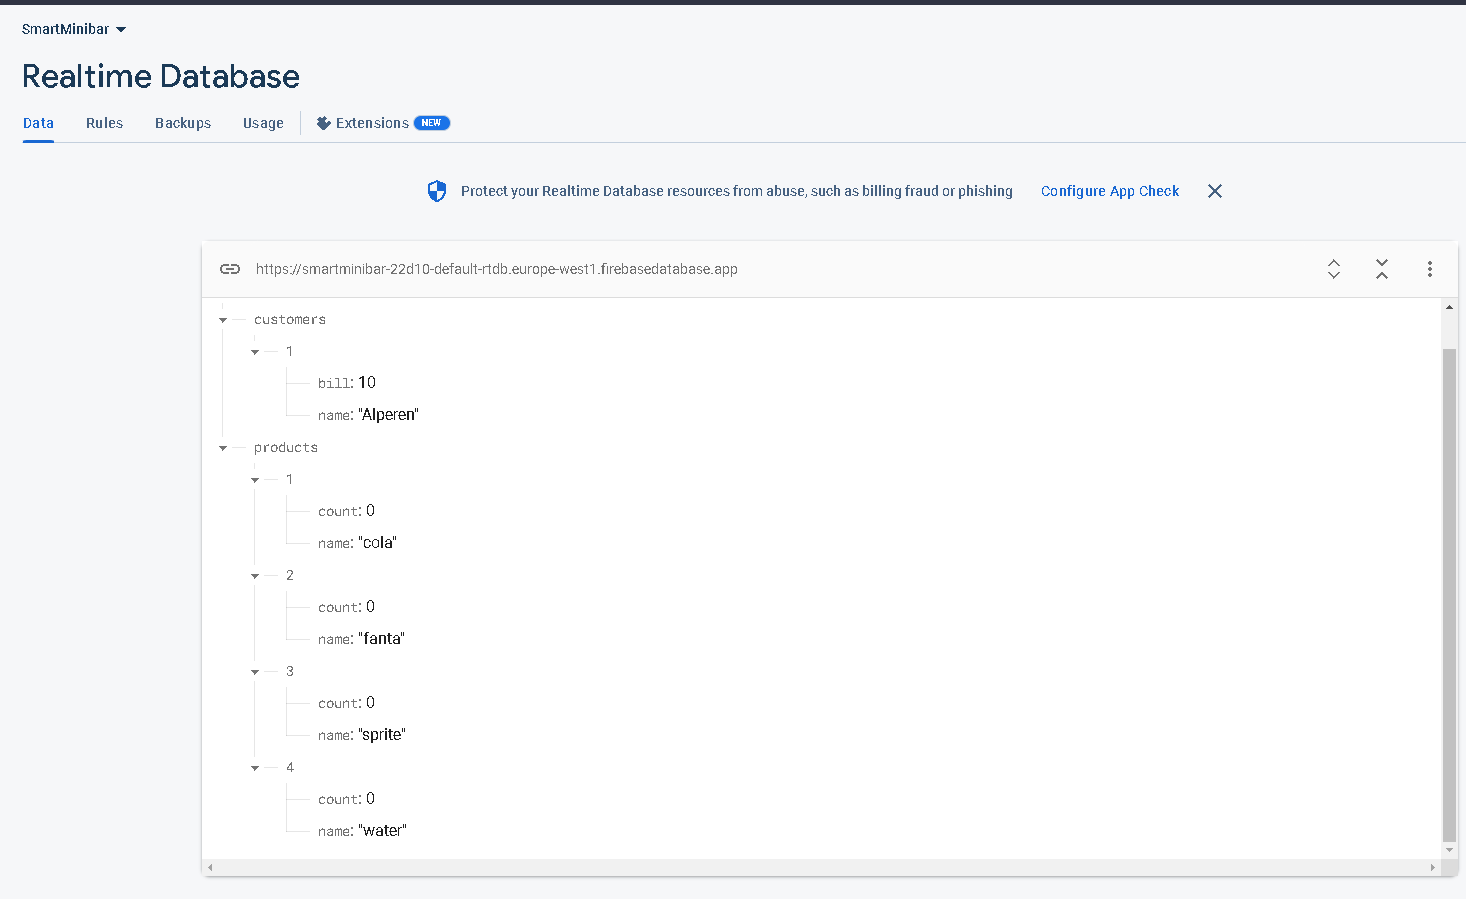
\includegraphics[width=0.8\textwidth]{Imgs/databasefirebase.png}
    \caption{\label{fig:Firabase}Firabase connection.}
\end{figure}
\\

\begin{figure}[!htbp]
    \centering
    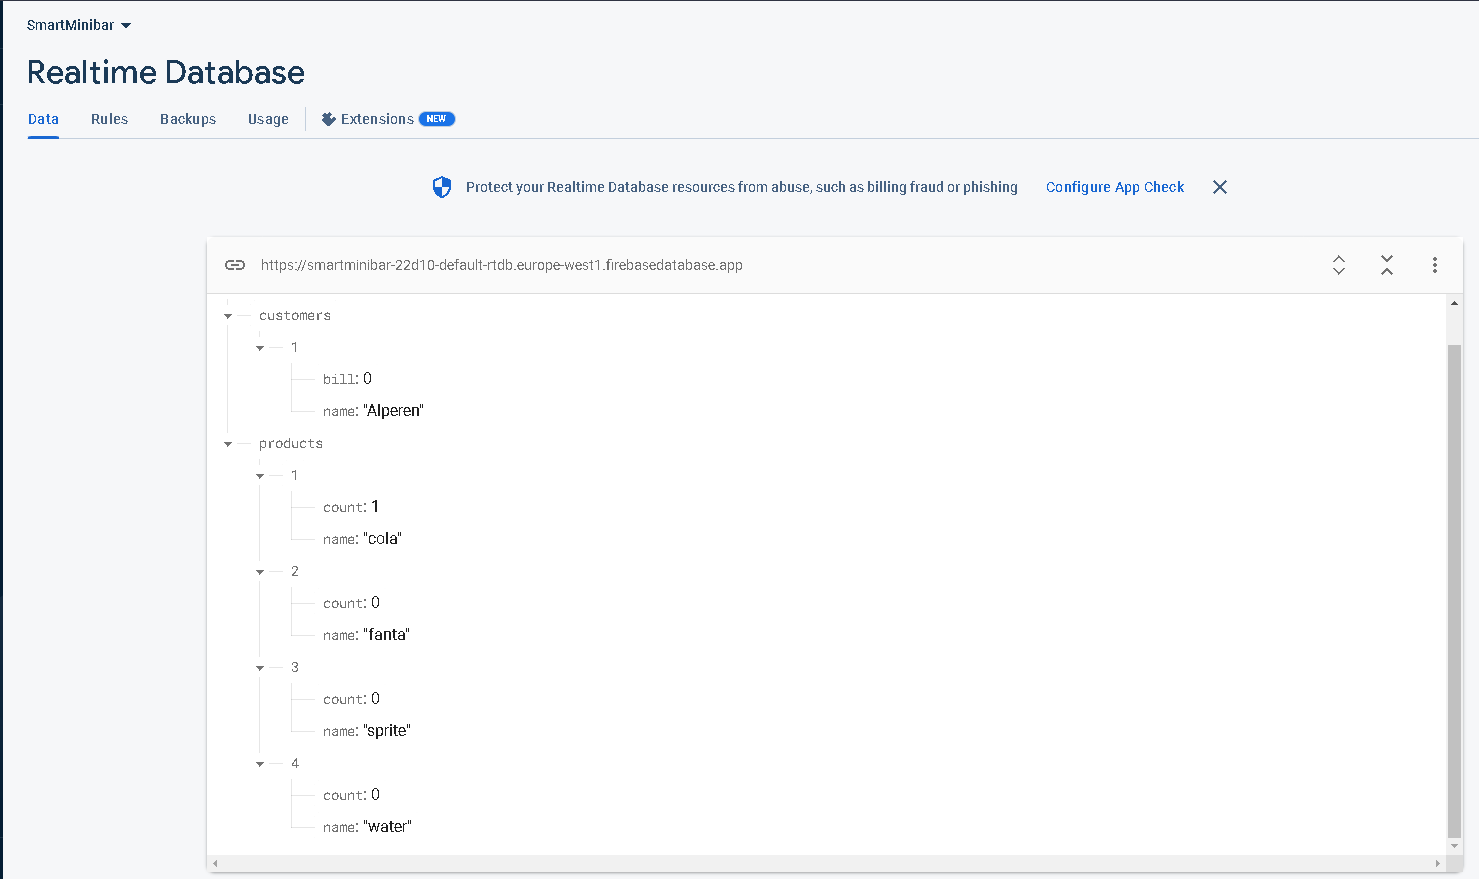
\includegraphics[width=0.8\textwidth]{Imgs/firebase1.png}
    \caption{\label{fig:Firabase}Firabase connection.}
\end{figure}
\\

This photos show when user takes 1 cola from minibar, what happens.